\documentclass{report}

% ----- IMPORTS ---------------------------------------------------------------
\usepackage[ngerman]{babel}
\usepackage{float}
\usepackage[ngerman]{datetime}
\usepackage[bookmarks]{hyperref} % PDF TOC
\usepackage{graphicx}
%\usepackage{baskervald} % Use the Baskerville font
\usepackage[utf8x]{inputenc}
\setcounter{secnumdepth}{5} % include numbering in paragraph heading

% ----- META ------------------------------------------------------------------
\title{Software Engineering\\\small{WS2015/2016}}
\author{
	\textsc{Tim Bierenbreier}\footnote{liebt \LaTeX}\\
	\normalsize Matrikel Nr.: 43235
	\and
	\textsc{Jonas Rottmann}\\
	\normalsize Matrikel Nr.: 44501
	\and
	\textsc{Jonas Weber}\\
	\normalsize Matrikel Nr.: 43399 \\[2cm]
	{\Huge Gruppe 24} \\[2cm]
}

% ----- CONTENT ---------------------------------------------------------------
\begin{document}

\maketitle

\tableofcontents

\chapter{Analyse}
\section{Use-Cases}
\textit{Beschreiben Sie jeden Use-Case (mindestens 5) mit eigenen Worten. Priorisieren Sie Ihre Use-Cases (essentiell, wichtig, unwichtig) und begr\"unden Sie Ihre Entscheidung.}
\begin{description}
   \item[Spielfeld vorbereiten]~\par
   \begin{description}
      \item[Akteure] Alle Spieler
      \item[Priorität] essentiell\\Grundlage für den weiteren Spielverlauf.
      \item[Beschreibung] Die Spieler bestimmen die 4 Kategorien. Jeder Spieler wählt eine Farbe. Die Wissensstreiter jedes Spielers werden auf die entsprechenden Heimatfelder gesetzt und die Wissenstandsanzeiger ggf. zurückgesetzt.
      \item[Vorbedingungen] Ein Spiel wird von den Spielern gestartet.
   \end{description}


   \item[Beginnenden Spieler bestimmen]~\par
   \begin{description}
      \item[Akteure] Alle Spieler
      \item[Priorität] unwichtig\\Im Entwicklungsprozess nicht wichtig, da der beginnende Spieler leicht ohne Nebenwirkungen manuell bestimmt werden kann.
      \item[Beschreibung] Alle Spieler würfeln einmal, die höchste Augenanzahl beginnt. Falls mehr als ein Spieler die höchste Zahl würfelt, müssen diese Spieler erneut gegeneinander würfeln.
      \item[Vorbedingungen] Es sind 2 bis 4 Spieler bekannt und es gibt einen Würfel.
   \end{description}


   \item[Zug spielen]~\par
   \begin{description}
      \item[Akteure] Ein Spieler
      \item[Priorität] essentiell\\Hauptbestandteil des Spiels.
      \item[Beschreibung] Das System würfelt für den Spieler. Wenn eine 6 fällt wird ein Wissenstreiter auf das Spielfeld (sein Startfeld - das Feld seiner Farbe) gebracht. Wurde keine 6 gewüfelt, oder sind bereits alle Wissensstreiter auf dem Feld, darf der Spieler einen seiner Wissensstreiter um die gewürfelte Augenzahl nach vorne ziehen. Kommt der Wissensstreiter des Spielers auf ein Feld, das von einem eigenen Wissensstreiter oder dem eines anderen Spielers besetzt ist, tritt der Use Case "`Wissen testen"' ein. Hat der Spieler keine Wissensstreiter auf dem Feld, darf maximal 3 mal gewürfelt werden bis eine 6 fällt. Wenn der Spielzug beendet wurde, ist der Spieler zu seiner Rechten am Zug.
      \item[Vorbedingungen] Ein Spieler ist am Zug.
   \end{description}


   \item[Wissen testen (extends "`Zug spielen"')]~\par
   \begin{description}
      \item[Akteure] Bis zu zwei Spieler
      \item[Priorität] essentiell\\Hauptbestandteil des Spiels.
      \item[Beschreibung] Spieler stellt anderem Spieler Frage aus einer der 4 Kategorien.\\
Frage wird korrekt beantwortet: Wissenstandsanzeiger dieser Kategorie wird inkrementiert. Wenn der Wissenstandszeiger dieser Kategorie auf höchster Stufe ist, kann eine beliebige andere Kategorie inkrementiert werden. Der Wissensstreiter des geprüften Spielers muss auf dessen Startfeld zurückgesetzt werden, ist dieses besetzt ins Heimatfeld.\\
Frage konnte nicht beantwortet werden: Der Wissenstandsanzeiger dieser Kategorie wird dekrementiert. Der Wissensstreiter des geprüften Spielers kommt ins Heimatfeld.
      \item[Vorbedingungen] Spieler kommt auf ein Feld auf dem ein Wissensstreiter steht (beliebige Farbe).
   \end{description}


   \item[Anderen Spieler testen (erbt von "`Wissen testen"')]~\par
   \begin{description}
      \item[Akteure] Zwei Spieler
      \item[Priorität] essentiell\\Hauptbestandteil des Spiels.
      \item[Beschreibung] Zusätzlich: Beantwortet der zu testende Spieler die Frage falsch, kann der Fragesteller selbst eine Frage der entsprechenden Kategorie beantworten.
      \item[Vorbedingungen] Feld ist von einem fremden Wissensstreiter belegt.
   \end{description}


   \item[Sich selbst testen (erbt von "`Wissen testen"')]~\par
   \begin{description}
      \item[Akteure] Ein Spieler
      \item[Priorität] unwichtig\\Kann bei funktionierendem Wissen testen einfach nach implementiert werden.
      \item[Beschreibung]
      \item[Vorbedingungen] Feld ist von einem eigenen Wissensstreiter belegt.
   \end{description}


   \item[Sieger bestimmen]~\par
   \begin{description}
      \item[Akteure] Spielleiter (Computer)
      \item[Priorität] unwichtig\\Für den Spielverlauf zuerst uninteressant.
      \item[Beschreibung] Zeige den Gewinner an und biete an eine neue Runde zu starten.
      \item[Vorbedingungen] Ein Spieler hat seine Wissenstandanzeige komplett gefüllt.
   \end{description}
\end{description}

\subsection{Use-Case Diagramm}
\textit{Skizzieren Sie das Use-Case-Diagramm mit allen Akteuren und Abh\"angigkeiten.}
\begin{figure}[H]
	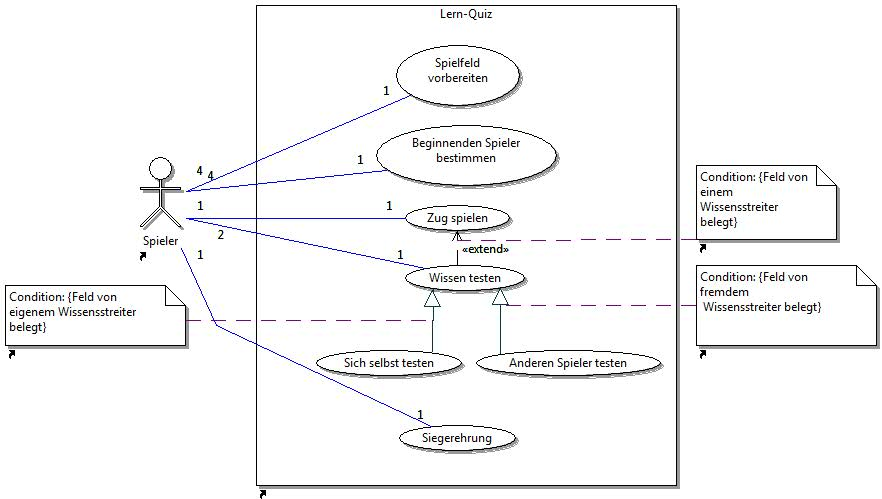
\includegraphics[width=\textwidth]{Diagramme/UseCaseDiagram.jpg}
	\centering
\end{figure}

\subsection{Erste Iteration}
\textit{Bestimmen Sie den Umfang der ersten Iteration (3 Use-Cases).}
\begin{itemize}
   \item Spiefeld vorbereiten
   \item Zug spielen
   \item Wissen testen
\end{itemize}

\section{Use-Cases, Details, Objektmodell und Schnittstellen der ersten Iteration}

\subsection{Aktivitäts Diagramme}
\textit{Erstellen Sie f\"ur die Use-Cases (obige 3) Beschreibungen in Form von Activity-Diagrammen.}

\begin{figure}[H]
	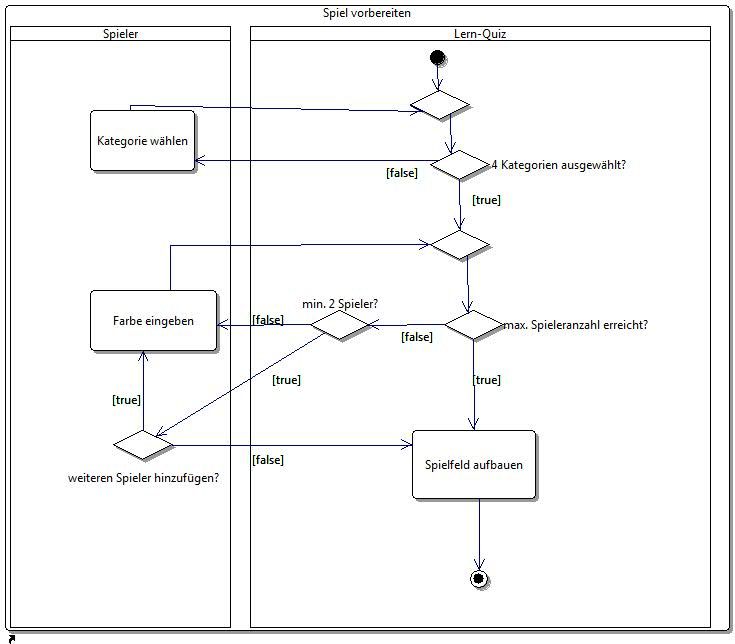
\includegraphics[width=\textwidth]{Diagramme/ActivityDiagram-SpielVorbereiten.jpg}
	\caption{Spiefeld vorbereiten}
	\centering
\end{figure}

\begin{figure}[H]
	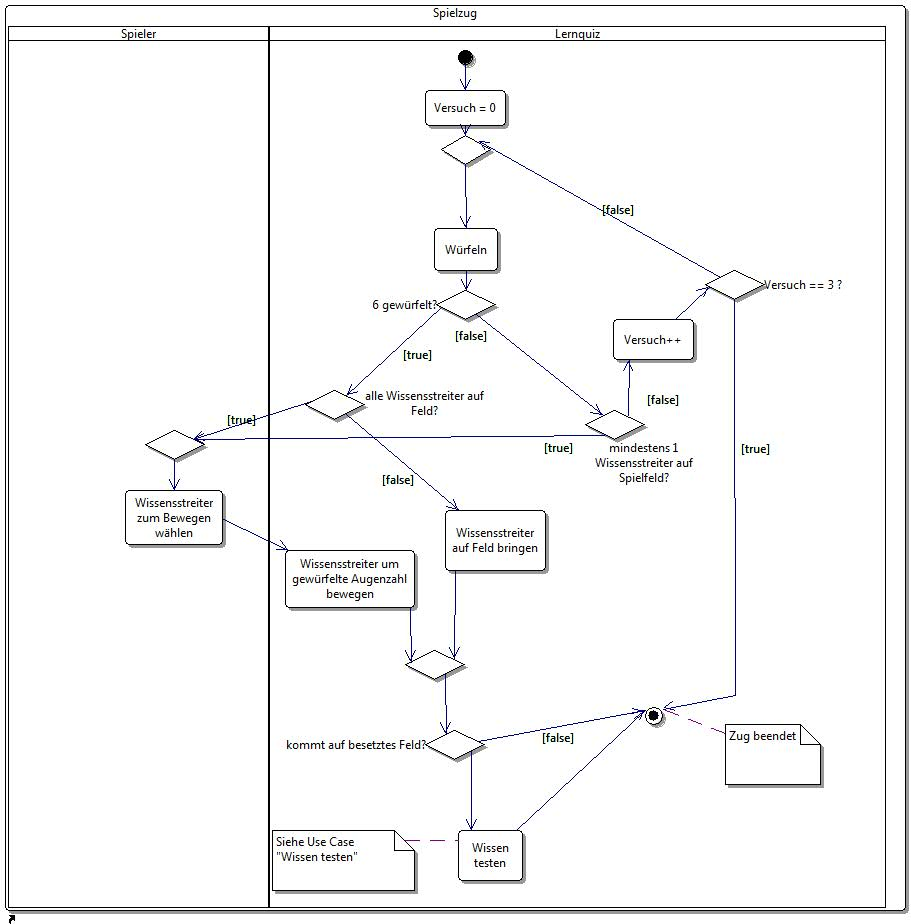
\includegraphics[width=\textwidth]{Diagramme/ActivityDiagram-Spielzug.jpg}
	\caption{Zug spielen}
	\centering
\end{figure}

\begin{figure}[H]
	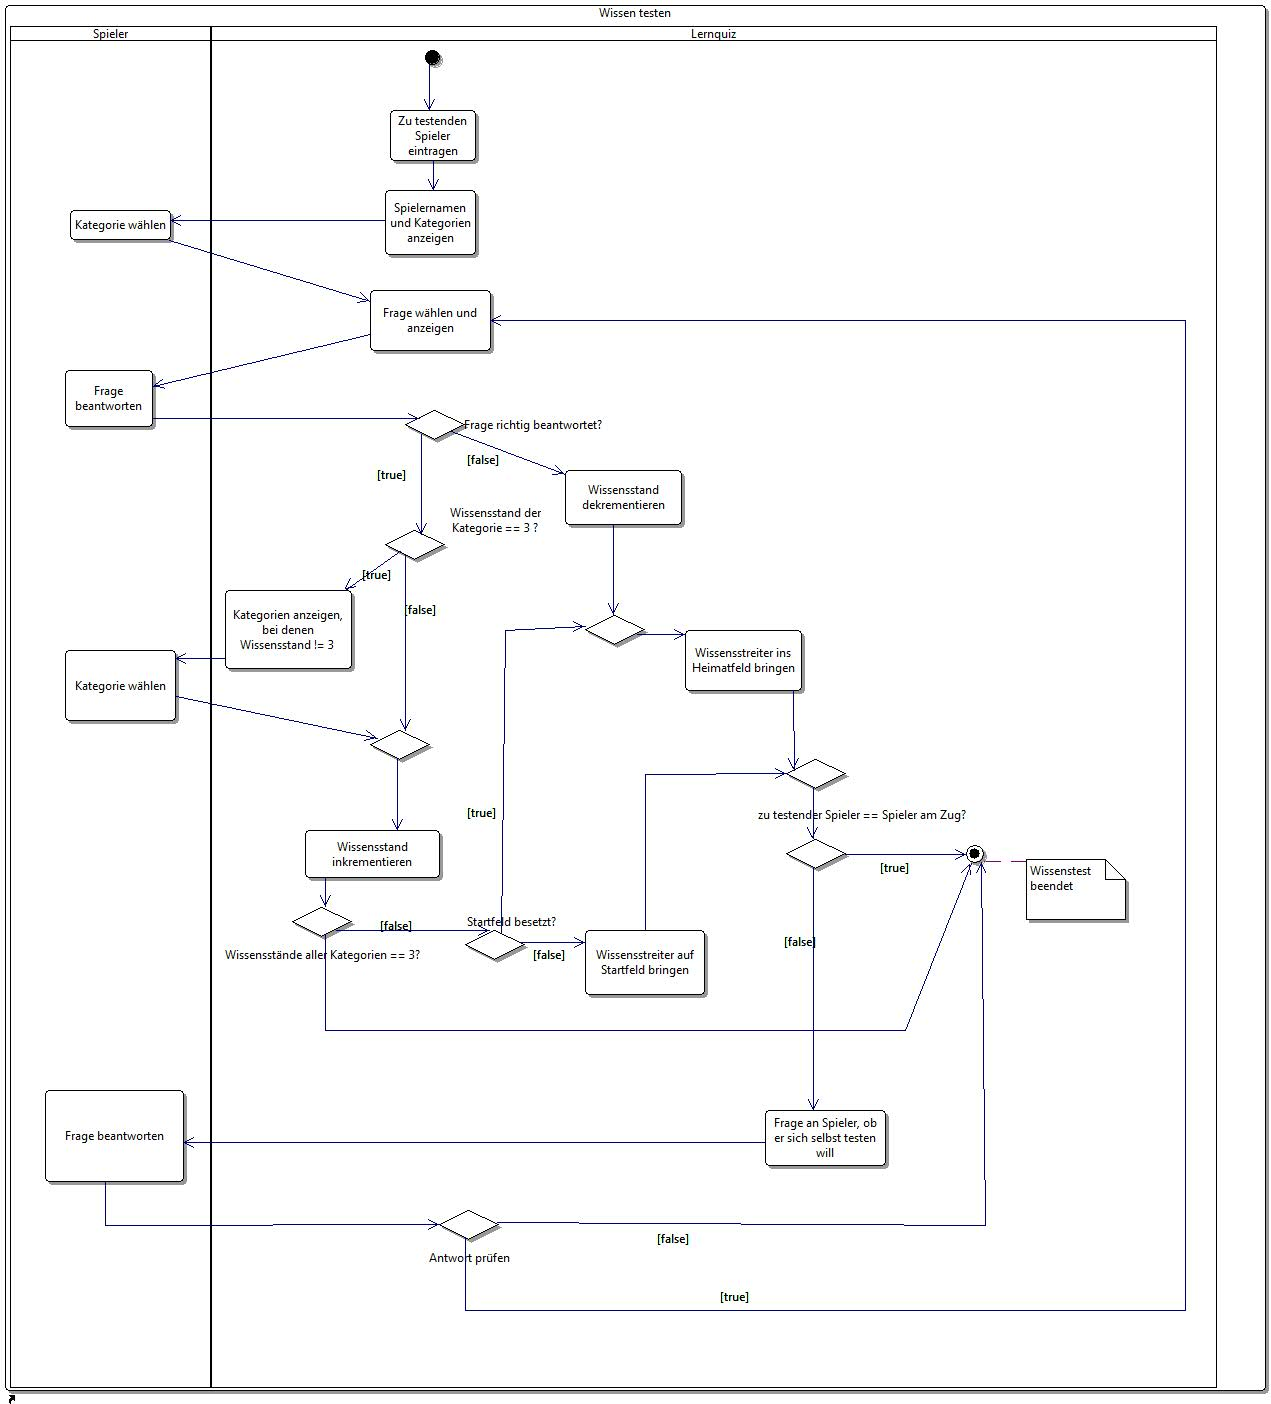
\includegraphics[width=\textwidth]{Diagramme/ActivityDiagram-WissenTesten.jpg}
	\caption{Wissen testen}
	\centering
\end{figure}


\subsection{Klassendiagramm}
\textit{Extrahieren Sie aus den erstellten Diagrammen die Konzepte des Lern-Quiz-Computer-Spiels und ihre Beziehungen. Stellen Sie diese in Form eines Klassendiagramms dar (Objektmodell).}
\begin{figure}[H]
	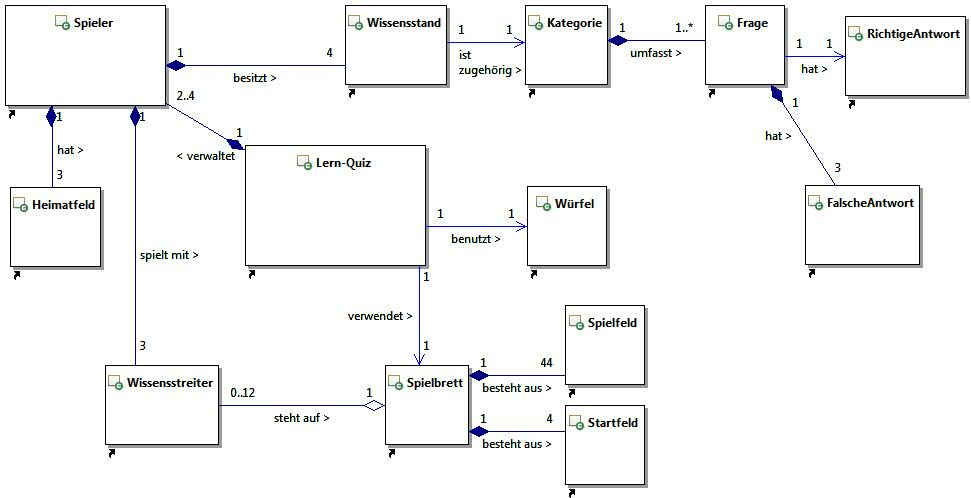
\includegraphics[width=\textwidth]{Diagramme/ClassDiagram.jpg}
	\caption{Klassen Diagramm}
	\centering
\end{figure}



\subsection{Systemoperationen}
\textit{Bestimmen Sie aus den Activity-Diagrammen die m\"oglichen Systemoperationen. Erstellen Sie zur besseren \"Ubersicht System-Sequenz-Diagramme und beschreiben Sie jede Operation mit eigenen Worten.}

\subsubsection{Spiel vorbereiten}
\begin{figure}[H]
	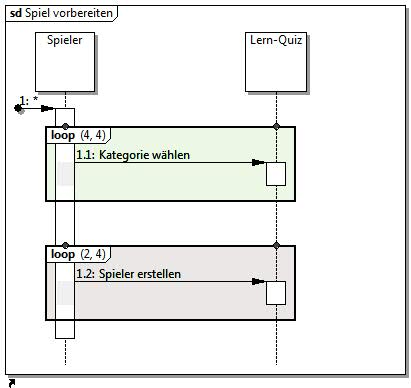
\includegraphics[width=\textwidth]{Diagramme/SequenceDiagram-SpielVorbereiten.jpg}
	\centering
\end{figure}

\paragraph{Kategorie wählen}
\begin{description}
	\item[Verantwortlichkeit] Ein Spieler wählt die Kategorien für die Fragerunden aus.
	\item[Bemerkungen] Um Komplexität zu verhindern wählt Spieler 1 die Kategorien aus.
	\item[Ausnahmen] Keine
	\item[Vorbedingungen] Ein neues Spiel wurde gestartet.
	\item[Nachbedingungen] Die Kategorien wurden im System dem neuen Spiel zugeordnet.
\end{description}

\paragraph{Spieler erstellen}
\begin{description}
	\item[Name] Spieler erstellen
	\item[Verantwortlichkeit] Für jeden Spieler (2 bis 4) wird im System ein Spieler registriert.
	\item[Bemerkungen] Keine
	\item[Ausnahmen] Keine
	\item[Vorbedingungen] Kategorien wurden gewählt.
	\item[Nachbedingungen] Das Spiel beginnt.
\end{description}



\subsubsection{Spielzug}
\begin{figure}[H]
	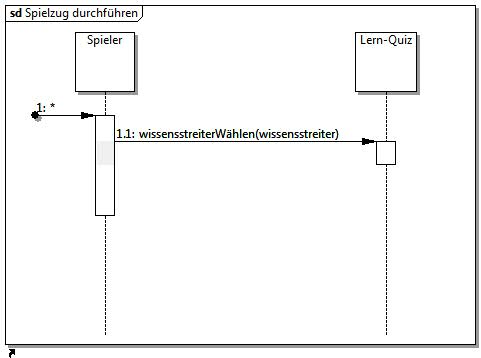
\includegraphics[width=\textwidth]{Diagramme/SequenceDiagram-Spielzug.jpg}
	\centering
\end{figure}

\paragraph{Zug starten}
\begin{description}
	\item[Verantwortlichkeit] Ein Spieler beginnt seinen Zug indem er würfelt.
	\item[Bemerkungen] Keine
	\item[Ausnahmen] Keine
	\item[Vorbedingungen] Der vorherige Spielzug wurde beendet und es wurde noch kein Gewinner ermittelt.
	\item[Nachbedingungen] Ein Wissensstreiter muss bewegt werden.
\end{description}

\paragraph{Wissensstreiter wählen}
\begin{description}
	\item[Verantwortlichkeit] Der Spieler wählt einen seiner Wissensstreiter aus und zieht ihn um n (n ≈ gewürfelte Augenzahl) Felder nach vorne.
	\item[Bemerkungen] Bei einer Augenanzahl kleiner 6 darf der Spieler jeden seiner auf dem Spielfeld befindlichen Wissensstreiter wählen und bewegen. Bei einer Augenanzahl von 6 muss der Spieler, falls noch nicht alle seiner Wissensstreiter auf dem Spielfeld sind einen Wissensstreiter aus seinem Heimatfeld auf sein Startfeld setzen.
	\item[Ausnahmen] Hat der Spieler keine Wissensstreiter auf dem Feld und hat keine 6 gewürfelt, darf er maximal 3 mal würfeln bis eine 6 fällt. Dann darf ein Wissensstreiter auf das Startfeld gesetzt werden.
	\item[Vorbedingungen] Der Spieler hat gewürfelt.
	\item[Nachbedingungen]
\end{description}



\subsubsection{Wissen testen}
\begin{figure}[H]
	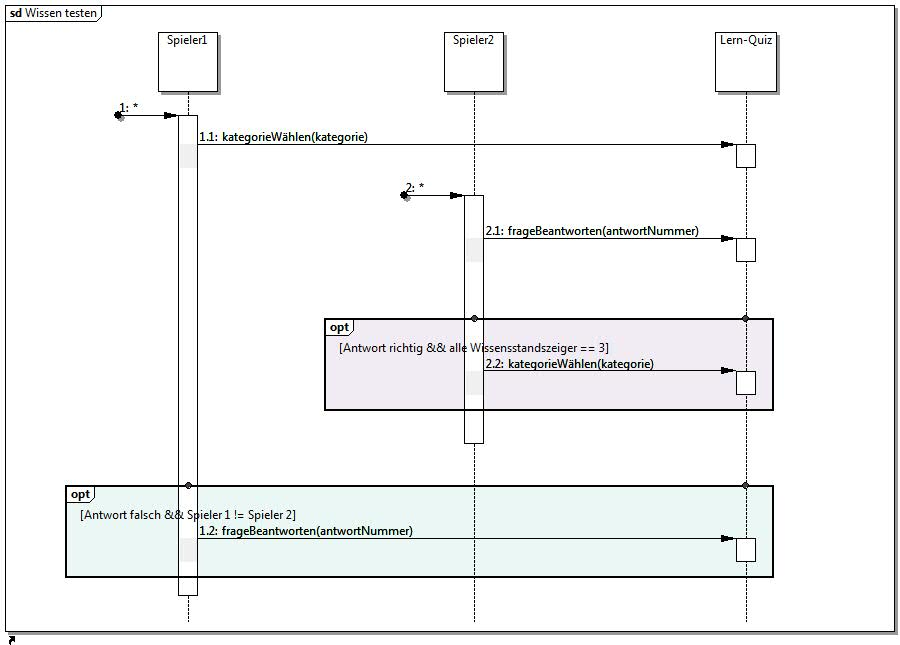
\includegraphics[width=\textwidth]{Diagramme/SequenceDiagram-WissenTesten.jpg}
	\centering
\end{figure}

\paragraph{Kategorie wählen}
\begin{description}
	\item[Verantwortlichkeit] Der testende Spieler wählt eine der 4 Kategorien.
	\item[Bemerkungen] Wurde die ursprüngliche Frage falsch beantwortet, erhält der Frgestelle die Möglichkeit selbst eine Kategorie für eine weitere Frage zu wählen, die er selbst beantworten muss.
	\item[Ausnahmen] Keine
	\item[Vorbedingungen] Ein Spieler zieht einen seiner Wissensstreiter auf ein Feld, das von einem Wissensstreiter besetzt ist.
	\item[Nachbedingungen] Die Frage muss beantwortet werden.
\end{description}

\paragraph{Frage beantworten}
\begin{description}
	\item[Verantwortlichkeit] Der Spieler beantwortet die Frage, die vom System gestellt wurde.
	\item[Bemerkungen] Keine
	\item[Ausnahmen] Keine
	\item[Vorbedingungen] Eine Kategorie wurde gewählt.
	\item[Nachbedingungen] Darauf wird die Position des Wissensstreiter und der Wissensstandanzeiger des Spielers verändert (siehe Use-Case "`Wissen testen"').
\end{description}

\chapter{Design}

\end{document}
